\chapter{Thực nghiệm}
\label{ch:thucnghiem}

\section{Thiết lập}

\paragraph{Dữ liệu.} 20 quỹ đạo thật (858 điểm) trích từ GeoLife
v1.3~\cite{zheng2010geolife}, giới hạn trong hộp tọa độ trung tâm Bắc Kinh
$(39{,}96;\,116{,}29)$--$(40{,}02;\,116{,}36)$, tách theo khoảng dừng, lấy mẫu
lại chu kỳ 20 giây (chế độ mà tương quan thời gian giữa hai điểm liên tiếp còn
mạnh --- đúng vùng hoạt động của tấn công HMM), mỗi quỹ đạo 20--60 điểm, tối đa
3 quỹ đạo mỗi người dùng.

\paragraph{Lưới đường.} Đồ thị OSM dựng từ extract BBBike cho cùng hộp tọa độ:
77.727 đỉnh, 208.994 cạnh. Toàn bộ tọa độ được chiếu về hệ phẳng cục bộ
(equirectangular quanh vĩ độ trung bình, sai số dưới 1m trong phạm vi 10km).

\paragraph{Cơ chế so sánh.} (1)~Laplace phẳng thuần (Geo-I
gốc~\cite{andres2013geo}, bán kính Gamma$(2,1/\eps)$, không chặn, không snap);
(2)~Baseline Thực tập 2 (nhiễu chặn tại QoS + làm mượt + snap có kiểm QoS);
(3)~REM; (4)~T-REM ($v_{\max} = 25$ m/s, $s = 100$m, $\lambda = 0{,}02$);
(5)~SM-REM (T-REM + memoization lưới công khai $g = 60$m).
QoS $\delta = 200$m; $\eps \in \{0{,}01;\, 0{,}02;\, 0{,}05\}$ mỗi mét; seed cố
định 42.

\section{Độ đo và tấn công}

\emph{Tiện ích:} độ lệch trung bình/lớn nhất giữa điểm thật và điểm công bố
(quality loss); tỷ lệ thỏa QoS; recall truy vấn k-NN POI (theo giao thức
của~\cite{xiao2015protecting}); khoảng cách Hausdorff và DTW giữa hai quỹ đạo.
\emph{Tính thực tế:} tỷ lệ điểm công bố nằm trong 25m của lưới đường; tỷ lệ cặp
điểm công bố liên tiếp vi phạm tốc độ 30 m/s.
\emph{Riêng tư:} sai số của \emph{adversary Bayes với emission REM chính xác}
--- prior đều cố định trên toàn tập đỉnh, likelihood
$\propto \exp(-\tfrac{\eps}{2}d(x,z))/Z(x)$ với normalizer $Z(x)$ tính đủ trên
toàn support, estimator là geometric median (khớp loss khoảng cách). Adversary
này \emph{chính xác} cho REM; với T-REM/SM-REM (likelihood phụ thuộc lịch sử/trạng
thái) nó là adversary REM-emission cố định áp dụng đồng nhất, \emph{không} tuyên
bố là Bayes-optimal riêng cho từng cơ chế. Kèm tấn công theo dõi HMM
(forward--backward, cùng emission có $Z(x)$, cột \emph{cov} = tỷ lệ đỉnh proxy của
vị trí thật còn trong tập ứng viên sau cắt). Sai số càng \emph{cao} càng riêng tư.

\section{Kết quả}

\begin{table}[ht]
\centering
\caption{Kết quả trên 20 quỹ đạo GeoLife (858 điểm), QoS 200m, seed 42. Bayes/HMM
err = sai số adversary (m), cao hơn là riêng tư hơn; cov = HMM candidate coverage.
In đậm: cơ chế đề xuất.}
\label{tab:benchmark}
\small
\begin{tabular}{llrrrrrrr}
\toprule
$\eps$ & Cơ chế & Q\_loss & QoS & On-road & Spd-viol & Bayes & HMM & cov\\
\midrule
0,01
 & Laplace phẳng & 205,6 & 0,59 & 0,58 & 0,08 & 201,4 & 131,1 & 1,00\\
 & Baseline TT2 (surrogate) &  94,9 & 0,99 & 0,97 & 0,00 &  93,8 &  81,2 & 1,00\\
 & \textbf{REM}      & 370,1 & 0,33 & 1,00 & 0,35 & 366,8 & 198,8 & 0,97\\
 & \textbf{T-REM}    & 285,2 & 0,40 & 1,00 & 0,06 & 282,4 & 185,0 & 0,99\\
 & \textbf{SM-REM}   & 325,0 & 0,32 & 1,00 & 0,05 & 322,2 & 253,1 & 0,99\\
\midrule
0,02
 & Laplace phẳng & 102,8 & 0,89 & 0,63 & 0,01 & 100,5 &  79,1 & 1,00\\
 & Baseline TT2 (surrogate) &  80,0 & 1,00 & 0,99 & 0,00 &  80,3 &  75,1 & 1,00\\
 & \textbf{REM}      & 183,9 & 0,62 & 1,00 & 0,06 & 182,4 & 122,4 & 1,00\\
 & \textbf{T-REM}    & 178,4 & 0,66 & 1,00 & 0,02 & 177,7 & 123,5 & 1,00\\
 & \textbf{SM-REM}   & 196,6 & 0,59 & 1,00 & 0,01 & 195,7 & 159,2 & 1,00\\
\midrule
0,05
 & Laplace phẳng &  41,1 & 1,00 & 0,68 & 0,00 &  43,0 &  37,8 & 1,00\\
 & Baseline TT2 (surrogate) &  68,8 & 1,00 & 0,99 & 0,00 &  69,6 &  68,8 & 1,00\\
 & \textbf{REM}      &  76,3 & 0,96 & 1,00 & 0,00 &  76,1 &  66,4 & 1,00\\
 & \textbf{T-REM}    &  76,9 & 0,95 & 1,00 & 0,00 &  76,9 &  67,3 & 1,00\\
 & \textbf{SM-REM}   &  75,7 & 0,97 & 1,00 & 0,00 &  75,5 &  69,2 & 1,00\\
\bottomrule
\end{tabular}
\end{table}

Năm quan sát chính từ Bảng~\ref{tab:benchmark} (số liệu với adversary emission
chính xác; đọc thận trọng, tránh overclaim):

\begin{enumerate}
  \item \textbf{Tương quan thời gian là mối đe dọa thực.} Tấn công HMM luôn
  mạnh hơn tấn công per-point: với Laplace phẳng tại $\eps = 0{,}01$, sai số
  adversary giảm từ 201,4m (Bayes) xuống 131,1m (HMM, $-35\%$) chỉ nhờ lọc Bayes
  theo thời gian --- xác nhận thực nghiệm~\cite{xiao2015protecting} và biện minh
  việc chọn HMM làm tấn công đánh giá chính.
  \item \textbf{Laplace phẳng để lộ bề mặt tấn công thực tế.} 32--42\% điểm công
  bố rơi ngoài lưới đường --- đúng loại tín hiệu mà RAoPT khai thác. REM/T-REM/
  SM-REM đạt 100\% trên đường \emph{theo cấu trúc} (đây là structural property,
  chưa phải bằng chứng attack-resistance --- cần chạy RAoPT trực tiếp, xem
  Chương~\ref{ch:tongket}).
  \item \textbf{T-REM giảm tín hiệu speed-implausibility nhưng KHÔNG "đóng"
  velocity attack.} Tại $\eps = 0{,}01$, T-REM giảm tỷ lệ vi phạm tốc độ từ 35\%
  (REM) xuống 6\% và \emph{đồng thời} giảm quality loss (370,1 $\to$ 285,2m).
  Nhưng theo chính metric HMM, T-REM (185,0m) cho adversary error \emph{thấp
  hơn} REM (198,8m) --- tức T-REM đánh đổi một chút riêng-tư-HMM lấy tính thực tế
  và tiện ích, chứ không loại bỏ tấn công. Đây là một soft regularizer theo
  khoảng cách đường thẳng, không phải hard reachable-set.
  \item \textbf{Trên đường cong trade-off, lợi thế của cơ chế đường là tính thực
  tế và guarantee hợp lệ, không phải attacker-error thô.} Tại mức tiện ích tương
  đương (Laplace @$\eps{=}0{,}01$ disp 205,6m, HMM 131,1m so với T-REM
  @$\eps{=}0{,}02$ disp 178,4m, HMM 123,5m), sai số HMM gần bằng nhau; cơ chế
  đường \emph{không} thắng trên trục attacker-error. Lợi thế thật của chúng là:
  100\% trên đường (không có bề mặt map-matching), 0\% vi phạm tốc độ, và
  $\eps$ là \emph{đảm bảo hợp lệ} --- khác với baseline có $\eps$ danh nghĩa đẹp
  nhưng theo Mệnh đề~\ref{prop:cap},~\ref{prop:reject} không phải guarantee hợp
  lệ (nên gọi là ``surrogate'' trong bảng).
  \item \textbf{SM-REM giữ hiệu năng trên quỹ đạo di chuyển và thêm chống
  averaging.} Trên trace GeoLife (đa số ô lưới riêng biệt), SM-REM bám sát T-REM
  về utility (disp 196,6 vs 178,4m tại $\eps{=}0{,}02$; quantize về $\mathrm{rep}(cell)$
  thêm chút lệch) và cho HMM error cao hơn (159,2 vs 123,5m). Lợi ích riêng của
  SM-REM --- chống averaging tại stay-point --- lộ ra ở Mục~\ref{sec:averaging},
  không ở bảng di chuyển này.
\end{enumerate}

\section{Tấn công averaging tại stay-point (S4)}
\label{sec:averaging}

Bảng~\ref{tab:benchmark} đo quỹ đạo \emph{di chuyển}. Nhưng harm thực tế nghiêm
trọng nhất (Strava lộ nhà 84--95\%~\cite{hassan2018run}; home fingerprinting của
broker) đến từ báo cáo \emph{lặp tại một điểm tĩnh}. Thí nghiệm minh hoạ dưới đây
cho một người dùng báo cáo $n$ lần từ đúng một điểm ``nhà'' (điểm đầu của quỹ đạo
GeoLife đầu tiên); kẻ tấn công lấy trung bình các điểm công bố, ta đo khoảng cách
từ ước lượng trung bình đến nhà thật.

\begin{table}[ht]
\centering
\caption{Tấn công averaging (một home, một seed, $\eps = 0{,}02$): khoảng cách (m)
từ ước lượng trung bình đến nhà thật, theo số lần báo cáo $n$. Đây là minh hoạ
\emph{cấu trúc}, không phải bằng chứng thống kê (xem chú thích).}
\label{tab:averaging}
\small
\begin{tabular}{lrrrrrr}
\toprule
Cơ chế & $n{=}1$ & $n{=}2$ & $n{=}5$ & $n{=}10$ & $n{=}50$ & $n{=}100$ \\
\midrule
Laplace phẳng & 104,6 & 123,8 & 48,5 & 35,7 & 24,5 & \textbf{12,4} \\
Baseline TT2  &  44,4 &  49,5 & 65,5 & 65,9 & 36,3 & 28,6 \\
REM           & 115,3 &  31,2 & 103,1 & 30,5 & 61,9 & 20,7 \\
T-REM         &  71,2 & 143,9 & 241,4 & 128,6 & 11,8 & 21,3 \\
\textbf{SM-REM} & 429,6 & 429,6 & 429,6 & 429,6 & 429,6 & \textbf{429,6} \\
\bottomrule
\end{tabular}
\end{table}

Điểm cần đọc đúng: với các cơ chế nhiễu độc lập, sai số adversary \emph{giảm} theo
$n$ (Laplace về 12,4m ở $n=100$ --- khôi phục nhà tới 12m; REM/T-REM cũng giảm
nhưng nhiễu hơn do full-support có đuôi nặng). Riêng \textbf{SM-REM phẳng tuyệt đối}
ở mọi $n$: mọi báo cáo trả về cùng một release đã memoize, nên trung bình của $n$
bản sao giống hệt không giảm phương sai. Đây là hệ quả \emph{tất định} của
Định lý~\ref{thm:smrem} (đúng cho vị trí tĩnh lặp lại), \emph{không} phải một
khẳng định thống kê về ``an toàn nhà'': giá trị phẳng 429,6m chỉ là một mẫu đơn ---
một home, một seed. Tính trên nhiều home/user/seed, error tại $n=100$ của SM-REM
dao động rộng (verifier V-005), và trung bình số học của các cơ chế đường hội tụ
về $\mathbb{E}[Z\mid x]$ (có thể lệch khỏi $x$), không nhất thiết về $x$. Đánh giá
đầy đủ đa-home với khoảng tin cậy và các radius có ý nghĩa là hướng phát triển
(Chương~\ref{ch:tongket}). Điều bảng này chứng minh chắc chắn: memoization loại bỏ
\emph{cơ chế} variance-reduction của averaging --- kịch bản S4 mà bản PTPPM
stateless~\cite{min2025road} bỏ ngỏ.

\section{Hệ thống mô phỏng và kịch bản sử dụng}
\label{sec:simulator}

Để minh họa trade-off một cách trực quan, chúng tôi xây dựng hệ thống mô phỏng
web (Hình~\ref{fig:simulator}) phát lại quỹ đạo GeoLife thật theo thời gian với
ba góc nhìn đồng thời: vị trí thật (chỉ người dùng thấy), điểm công bố (thứ duy
nhất máy chủ LBS nhận được), và ước lượng của kẻ tấn công HMM trực tuyến kèm sai
số từng bước. Trên đó chạy một truy vấn LBS cụ thể --- ``3 hiệu thuốc gần tôi
nhất'' --- phát tại điểm công bố và được chấm điểm so với đáp án đúng, cho thấy
QoS bằng con số theo từng giây.

\begin{figure}[ht]
\centering
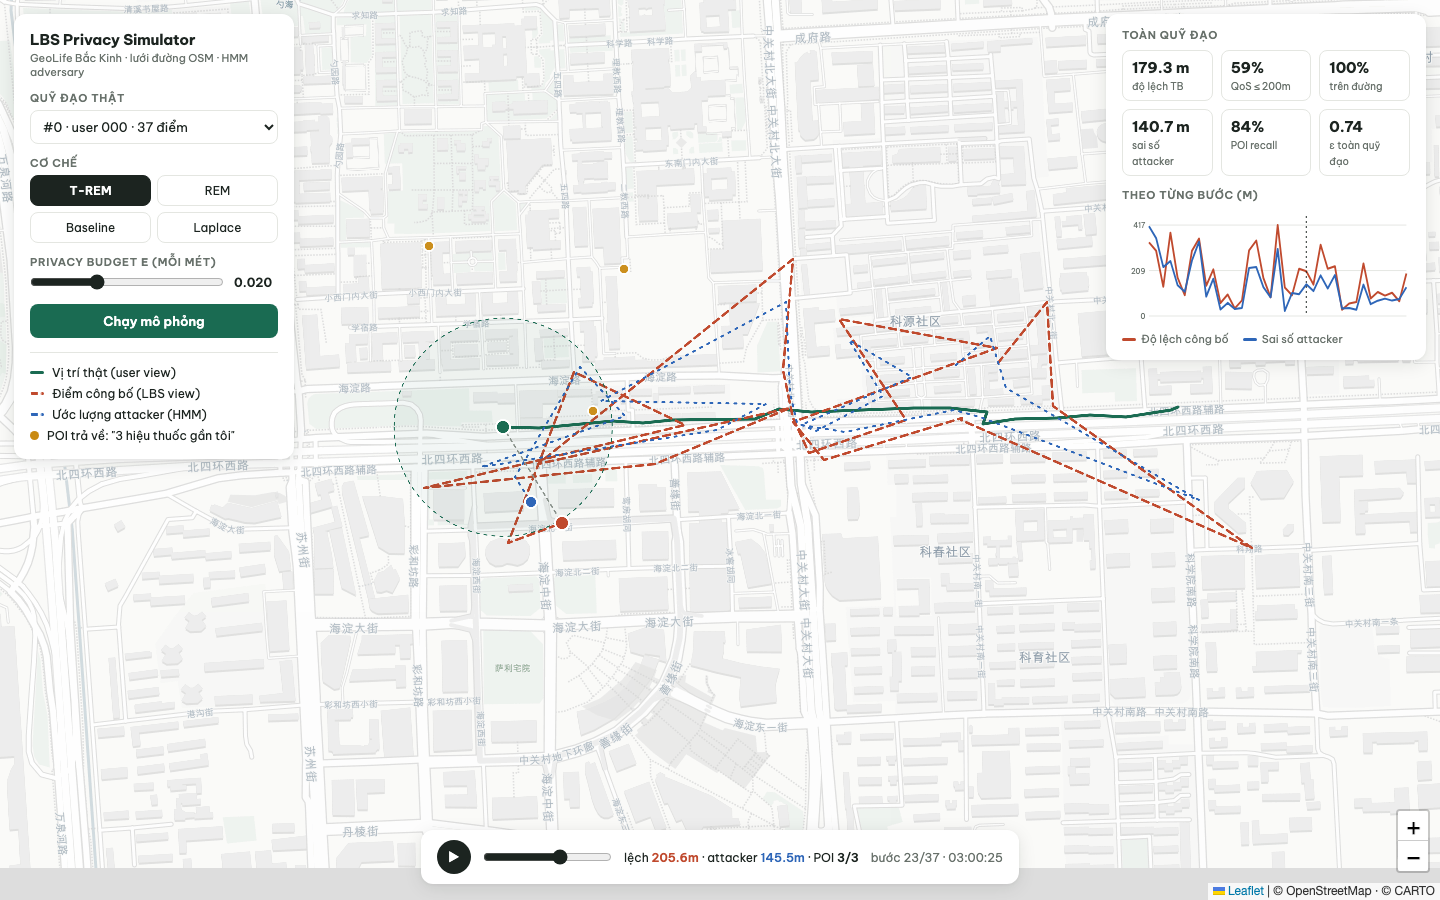
\includegraphics[width=\textwidth]{figures/simulator.png}
\caption{Hệ thống mô phỏng: quỹ đạo thật (xanh lá), chuỗi điểm công bố bởi T-REM
(đỏ, nét đứt), ước lượng kẻ tấn công HMM (xanh dương), vòng tròn QoS 200m, các
POI trả về từ truy vấn k-NN, bảng chỉ số toàn quỹ đạo và đồ thị sai số theo
từng bước.}
\label{fig:simulator}
\end{figure}

Bốn kịch bản đời thực được mô hình hóa: \emph{(i) gọi xe/giao đồ ăn} --- ứng
dụng cần vị trí thô để điều phối nhưng không được học địa chỉ nhà; \emph{(ii) y
tế nhạy cảm} --- tìm nhà thuốc gần mà không tiết lộ đang đứng trước phòng khám
nào (recall k-NN $\approx 81\%$ tại $\eps = 0{,}02$); \emph{(iii) ứng dụng thể
thao/mạng xã hội} --- chia sẻ tuyến chạy không lộ điểm xuất phát cho kẻ theo
dõi; \emph{(iv) crowdsensing giao thông} --- đóng góp dữ liệu tốc độ mà không
nộp nguyên hành trình, điểm công bố nằm trên lưới đường nên vẫn map-match được
cho mục đích thống kê.
